%%%%%%%%%%%%%%%%%%%%%%%%%%%%%%%%%%%%%%%%%
% University Assignment Title Page
% LaTeX Template
% Version 1.0 (27/12/12)
%
% This template has been downloaded from:
% http://www.LaTeXTemplates.com
%
% Original author:
% WikiBooks (http://en.wikibooks.org/wiki/LaTeX/Title_Creation)
%
% License:
% CC BY-NC-SA 3.0 (http://creativecommons.org/licenses/by-nc-sa/3.0/)
%
% Instructions for using this template:
% This title page is capable of being compiled as is. This is not useful for
% including it in another document. To do this, you have two options:
%
% 1) Copy/paste everything between \begin{document} and \end{document}
% starting at \begin{titlepage} and paste this into another LaTeX file where you
% want your title page.
% OR
% 2) Remove everything outside the \begin{titlepage} and \end{titlepage} and
% move this file to the same directory as the LaTeX file you wish to add it to.
% Then add \input{./title_page_1.tex} to your LaTeX file where you want your
% title page.
%
%%%%%%%%%%%%%%%%%%%%%%%%%%%%%%%%%%%%%%%%%
%\title{Title page with logo}
%----------------------------------------------------------------------------------------
%	PACKAGES AND OTHER DOCUMENT CONFIGURATIONS
%----------------------------------------------------------------------------------------

\documentclass[12pt]{article}
\usepackage[toc,page]{appendix}
\usepackage[spanish]{babel}
\usepackage[utf8x]{inputenc}
\usepackage{pgfplots}
\usepackage{amsmath}
\usepackage{graphicx}
\usepackage{fancyhdr}
\usepackage[colorinlistoftodos]{todonotes}
\usepackage{changepage}
\usepackage[font=scriptsize]{caption}
\usepackage[a4paper,bindingoffset=0.2in,left=1in,right=1in,top=1in,bottom=0.5in,footskip=.25in]{geometry}
\usepackage{cleveref}
\usepackage[hidelinks]{hyperref}
\usepackage{eurosym}
\usepackage{MathUnicode}
\usepackage{amssymb}
\usepackage{amsthm}
\usepackage{pdfsync}
\usepackage{color,xspace,hyperref}
\usepackage{changepage}
\usepackage{float}
\usepackage{caption}
\usepackage{titlesec}
\newcommand{\sectionbreak}{\clearpage}


\setlength{\arrayrulewidth}{1mm}
\setlength{\tabcolsep}{18pt}
\renewcommand{\arraystretch}{1.5}


\renewcommand{\labelitemii}{$\circ$}
\pagestyle{fancy}
\lhead{\textbf{Teoría del caos y fractales}}
%\chead{\leftmark}
\rhead{\leftmark}
%\rhead{\includegraphics[width=2.8cm]{img/logo_memo}}
%\rhead{\textbf{CyC}}

\newtheorem{theorem}{Teorema}[section]
\newtheorem{lemma}{Lema}[section]
\newtheorem{proposition}{Proposición}[section]
\theoremstyle{definition}
\newtheorem{definition}{Definición}[section]
\newtheorem{example}{Ejemplo}[section]

\renewcommand{\headrulewidth}{0.5pt}


\begin{document}

\begin{titlepage}

\newcommand{\HRule}{\rule{\linewidth}{0.5mm}} % Defines a new command for the horizontal lines, change thickness here

\center % Center everything on the page

%----------------------------------------------------------------------------------------
%	HEADING SECTIONS
%----------------------------------------------------------------------------------------

\textsc{\LARGE Universidad Autónoma de Madrid}\\[1.5cm] % Name of your university/college
\textsc{\Large Complejidad y Computación}\\[0.5cm] % Major heading such as course name


%----------------------------------------------------------------------------------------
%	TITLE SECTION
%----------------------------------------------------------------------------------------

\HRule \\[0.4cm]
{ \huge \bfseries Teoría del Caos y fractales}\\[0.4cm] % Title of your document
\HRule \\[1cm]


%----------------------------------------------------------------------------------------
%	AUTHOR SECTION
%----------------------------------------------------------------------------------------


% If you don't want a supervisor, uncomment the two lines below and remove the section above
\Large \emph{Autoress:}\\
Alejandro \textsc{Villegas}\\ % Your name
Elena \textsc{Gutiérrez}\\ % Your name
Miguel Ángel \textsc{González-gallego} \\
Pedro \textsc{Valero}\\[1cm] % Your name

%----------------------------------------------------------------------------------------
%	LOGO SECTION
%----------------------------------------------------------------------------------------

\includegraphics{img/Logo.jpg}\\ % Include a department/university logo - this will require the graphicx package

%----------------------------------------------------------------------------------------
%	DATE SECTION
%----------------------------------------------------------------------------------------

{\large \today}\\[1cm] % Date, change the \today to a set date if you want to be precise


%----------------------------------------------------------------------------------------

\vfill % Fill the rest of the page with whitespace

\end{titlepage}

\tableofcontents
\newpage

\section{Introducción}
Antes de comenzar a indagar en los fundamentos de la Teoría del Caos o en los fractales, debemos aclarar una serie de conceptos que aparecerán a lo largo de estos apuntes.

\begin{definition}[Sistema dinámico]\label{def:sistemaDinamico}
Un sistema dinámico es un sistema cuyo estado evoluciona con el tiempo. Los sistemas físicos en situación no estacionaria son ejemplos de sistemas dinámicos, pero también existen modelos económicos, matemáticos y de otros tipos que son sistemas abstractos que son sistemas dinámicos.

Según las variables que intervienen en el sistema sean \textbf{discretas} (sólo tomen una serie de valores posibles) o \textbf{continuas} (pueden tomar cualquier valor dentro de un intervalo), así lo será el sistema.
\end{definition}

Un sistema dinámico se define como \textbf{determinista} si existe una ecuación que nos permite conocer \emph{teóricamente} la evolución del sistema con total precisión.

\begin{definition}[Teoría del Caos]
La teoría del Caos es la rama de las Matemáticas que estudia el comportamiento de sistemas dinámicos \emph{deterministas} muy sensibles a los datos iniciales.
\end{definition}

Es importante destacar el hecho de que los sistemas han de ser deterministas pues, de lo contrario, estaríamos hablando de procesos aleatorios o impredecibles. La \emph{idea clave} del concepto del Caos es que comprendemos el fenómeno y sabemos modelizarlo ``a la perfección'' pero el resultado futuro varía enormemente a partir de un pequeño cambio en los valores tomados del mundo real.

\begin{example}
A modo de ejemplo podemos suponer un fenomeno que venga modelizado por la ecuación:
\[z_{n+1} = f(z_n) \text{ siendo } f(x) = x^2+1\]

Puesto que conocemos la ecuación que modela el fenómeno, queda claro que no encontramos ante un sistema dinámico determinista, pues para todo valor de $n$ podemos calcular $z_{n+1}$.

Para un $n=11$, que no parece ser algo demasiado grande, siendo $z$ un número complejo, supongamos que cometemos un error muy pequeño, de la forma: $ε=10^{-5}+10^{-5}i$ al medir $z_0$.

En estas condiciones, la diferencia entre el valor obtenido y el original es
\[f^{11}(ε)=1.4 \cdot 10^{181} + 1.13\cdot 10^{174}\]

Este ejemplo será estudiado con más detalle al hablar de los conjuntos de Mandelbrot
\end{example}

También es fundamental aclarar, aunque algunos lectores pueden tener ya una idea intuitiva, qué es un fractal.

\begin{definition}[Fractal]
Un fractal es un objeto geométrico cuya estructura básica, fragmentada o irregular, se repite a diferentes escalas.
\end{definition}

\section{Sistemas discretos}
Tiempo estimado de esta parte: 50 min\\
Referencia
\begin{itemize}
\item The Beauty of fractals temas 1,2,3,4 y 8.
\end{itemize}


\subsection{Ecuaciones en diferencias.}
% Pedro: Esta no es mi parte pero he escrito esto y al final me he dado cuenta de que se corresponde con sistemas discretos, no continuos. Así que lo pongo por aquí.

\begin{definition}[Ecuación en diferencias]
Una ecuación en diferencias es una expresión del tipo:
\[G(n,f(n),f(n+1),...,f(n+k))=0, \ \forall n \in \mathbb{Z}\]
donde $f$ es una función definida en $\mathbb{Z}$.
\end{definition}

\begin{example}
La ecuación en diferencias de primer orden:
\[X_{t+1} = F(X_t)\]
constituye un ejemplo de sistema dinámico determinista, siendo $F(x)$ una función conocida.
\end{example}


% Todo lo que viene a continuación viene de http://ltcconline.net/greenl/courses/204/firstOrder/differenceEquations.htm

A simple vista puede parecer que el ejemplo mencionado no es una ecuación en diferencias, puesto que no se aprecia ninguna derivada en la ecuación. No obstante, podemos escribir:
\[X'(t)=g(X(t)) \implies \lim_{h\to 0} \frac{X(t+h)-X(t)}{h}\]

Puesto que los valores posibles de $t$ y $h$ son enteros, lo más pequeño que puede ser $h$ sin llegar a ser $0$ es $h=1$ con lo que tenemos:
\[g(X(t))=X'(t)=X(t+h)-X(t)=ΔX(t) \implies X(t+h) = X(t) +ΔX(t) \implies \atop F(X(t)) = X(t) + ΔX(t)\]

Por tanto, encontrar la función $X(t)$ que resuelve el sistema planteado en el ejemplo es equivalente a resolver la ecuación:
\[X(t+1)=X(t)+ΔX(t)\]
que, claramente, es una ecuación en diferencias.

\subsection{Procesos de Verhulst. Period doubling, bifurcaciones.}
\subsection{Ecuación logística}
\subsection{$x=x^2+c$. Julia sets. Mandelbrot set.}
\subsection{Fractales/dimensión de Hausdorlf/dimensión fractal}
\subsection{Polvo de Cantor} No aparece en The Beauty of fractals (en algún otro libro de la bibliografía está).
\subsection{Ecuaciones de Volterra}

%%%%%%%%%%%%%%%%%%%%%%%%%%%%%%%%%%%%%%%%%%%%%%%%%%%%%%%%%%
%%%%%%%%%%%%%%%%%%%%%%%%%%%%%%%%%%%%%%%%%%%%%%%%%%%%%%%%%%
%%%%%%%%%%%%%%%%%%%%%%%%%%%%%%%%%%%%%%%%%%%%%%%%%%%%%%%%%%
%%%%%%%%%%%%%%%%%%%%%%%%%%%%%%%%%%%%%%%%%%%%%%%%%%%%%%%%%%
%%%%%%%%%%%%%%%%%%%%%%%%%%%%%%%%%%%%%%%%%%%%%%%%%%%%%%%%%%
%%%%%%%%%%%%%%%%%%%%%%%%%%%%%%%%%%%%%%%%%%%%%%%%%%%%%%%%%%
%%%%%%%%%%%%%%%%%%%%%%%%%%%%%%%%%%%%%%%%%%%%%%%%%%%%%%%%%%
%%%%%%%%%%%%%%%%%%%%%%%%%%%%%%%%%%%%%%%%%%%%%%%%%%%%%%%%%%
%%%%%%%%%%%%%%%%%%%%%%%%%%%%%%%%%%%%%%%%%%%%%%%%%%%%%%%%%%

\section{Sistemas continuos}
% Tiempo estimado de esta parte: 70 min.\\
% Referencia
% \begin{itemize}
% \item CHAOS: An introduction to dynamical systems temas 7,8,9 y 11.
% \item Elegant Chaos
% \end{itemize}

\subsection{Sistemas dinámicos deterministas, ecuaciones diferenciales}

Los sistemas dinámicos continuos deterministas, definidos en \ref{def:sistemaDinamico}, vienen modelizados por ecuaciones diferenciales.

En lugar de expresar el estado actual en función de un estado anterior, las ecuaciones diferenciales tratan de expresar la \emph{tasa de cambio} del estado actual en función del estado actual. La tasa de cambio de una cierta función es su \emph{derivada}. Tenemos la siguiente definicón general de ecuación diferencial.

\begin{definition}[Ecuación diferencial]
Una ecuación diferencial es una fórmula matemática que relaciona una función con sus derivadas.
\end{definition}

\begin{example}[Ecuación del calor]\label{ex:calor}
Un ejemplo de este tipo de dependencia es la \emph{Ley del calor de Newton}. Si consideramos $x$ como la diferencia de temperatura entre el objecto caliente y la temperatura ambiente del aire que lo rodea, la tasa de cambio de esta diferencia de temperatura es inversamente proporcional a la diferencia de temperatura. En términos de ecuaciones diferenciales, diremos:
\begin{equation}
x'(t) = ax(t)~~~con~~ a<0
\end{equation}

La solución de esta ecuación viene dada por:
\begin{equation}
x(t) = c\cdot e^{at}
\end{equation}

Esto quiere decir que la diferencia de temperatura $x(t)$ decrece exponencialmente con el tiempo $t$. Se trata de una ecuación  de \emph{primer orden}, puesto que el \emph{orden} de la derivada más alto que aparece es el de la \emph{primera} derivada, y \emph{lineal} porque la relación entre las funciones $x'(t)$ y $x(t)$ en la ecuación es \emph{lineal}.
\end{example}

En el siguiente ejemplo, veremos un caso de ecuación diferencial \emph{de segundo orden} \emph{no lineal}.

\begin{example}[Péndulo]
En este caso estudiaremos el movimiento de un péndulo \emph{bob}, el movimiento de un péndulo que tiene en su extrem un peso y que cuelga de un soporte que limita su movimiento a lo largo de un círculo. La aceleración que experimenta este péndulo es tangente a la dirección del movimiento y proporcional a la componente de la fuerza gravitatoria sobre la dirección tangencial. Si representamos con $x(t)$ la posición angular (es decir, la razón entre la longitud del arco que forma el péndulo con la vertical y la longitud del péndulo), entonces la relación entre su derivada segunda y ésta viene dada por:
\begin{equation}
x''(t) = -\sin x(t)
\end{equation}

Esta ecuación es una de las más importantes en ciencia y se trata de una ecuación de \emph{segundo orden}, puesto que el \emph{orden} de la derivada más alto que aparece es el de la \emph{segunda} derivada, y \emph \emph{no lineal}, porque la relación entre las funciones $x''(t)$ y $x(t)$ en la ecuación es \emph{no lineal}.
\end{example}


En ambos ejemplos, buscamos soluciones de la forma $x(t)$ donde $t$ denota el tiempo y $x(t)$, por tanto, una cierta magnitud física que varía en función del tiempo: en el primer ejemplo, la diferencia de temperatura; en el segundo ejemplo, la posición angular. Es por eso que consideramos que $x(t)$ es una variable \emph{dependiente}.


\begin{definition}[Ecuación diferencial autónomas]
Si la variable \emph{independiente} $t$ no aparece explicítamente en la ecuación, como es el caso en los dos ejemplos anteriores, hablaremos de ecuaciones diferenciales \textbf{autónomas}. Si $t$ aparece explícitamente en la ecuación como es el caso de la ecuación del \emph{péndulo amortiguado} (el columpio):
\begin{equation}
x''(t) = -cx'(t)-\sin x(t)+\rho~\sin t
\end{equation}
entonces hablaremos de ecuaciones diferenciales \textbf{no autónomas}.
\end{definition}

Recapitulando las nociones vistas hasta ahora tendríamos la siguiente clasificación de las ecuaciones diferenciales:

\begin{itemize}
\item Según el orden de las derivadas que aparezcan en la expresión:
	\begin{itemize}
	\item Primer orden
	\item Segundo orden
	\item ...
	\end{itemize}
\item Según la relación entre la función $x$ y sus derivadas
	\begin{itemize}
	\item Lineales
	\item No lineales
	\end{itemize}
\item Según si aparece explicítamente la variable $t$ en la ecuación
	\begin{itemize}
	\item Autónomas
	\item No autónomas
	\end{itemize}
\end{itemize}

Si recuperamos el ejemplo \ref{ex:calor}, teníamos que las soluciones eran de la forma:
\begin{equation}
x(t) = c \cdot e^{at}
\end{equation}

La $c$ es una constante en $\mathbb{R}$, cuyo valor dependerá del punto inicial que tomemos, es decir, la ecuación diferencial planteada en \ref{ex:calor} tiene \emph{infinitas} soluciones, a menos que especifiquemos un \emph{valor inicial} $x(0)$.

En el momento en que definimos un valor inicial $x(0)=x_0$ tenemos:
\[x(0)=c\cdot e^0=c \implies c=x_0 \implies x(t) = x(0)\cdot e^{at}\]

Así, estamos \emph{seleccionando} una de las soluciones dentro de la familia de soluciones.


% No se que aparece en la pagina que decías, pero yo me dibujo aquí la familia de funciones que creo que hay que poner xd
\begin{center}
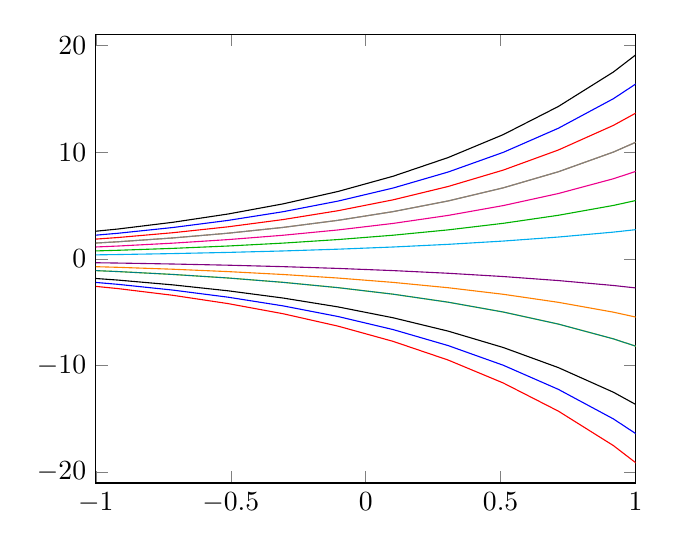
\begin{tikzpicture}
\begin{axis}[xmin=-1, xmax=1, samples=50, cycle list name=color list]
  \addplot (x,-7*e^x);
  \addplot (x,-6*e^x);
  \addplot (x,-5*e^x);
  \addplot (x,-3*e^x);
  \addplot (x,4*e^x);
  \addplot (x,-3*e^x);
  \addplot (x,-2*e^x);
  \addplot (x,-1*e^x);
  \addplot (x,e^x);
  \addplot (x,2*e^x);
  \addplot (x,3*e^x);
  \addplot (x,4*e^x);
  \addplot (x,5*e^x);
  \addplot (x,6*e^x);
  \addplot (x,7*e^x);
\end{axis}
\end{tikzpicture}
\captionof{figure}{Familia de funciones de la forma $x(t)=x(0)e^t$}
\end{center}

En nuestro caso, podemos establecer:

\begin{equation}
x(0) = x_0
\end{equation}

y por tanto, la solución particular de nuestro problema sería:

\begin{equation}
x(t) = x_0e^{at}.
\end{equation}

En general, a los problemas experesados en forma de ecuación diferencial más dato inicial, los denominaremos \textbf{problemas de valor inicial}.

A seguir con:

\begin{itemize}
\item Hablar de ls GRAFICA FAMILIA DE SOLUCIONES DE E. NO LINEALES (p.279)
\item Concepto de solución de equilibrio
\item Concepto de trayectorias/puntos atractores
\item Concepto de trayectorias/puntos ?repelentes?
\item Concepto de existencia, unicidad y dependencia continua (que no es lo mismo que dependencia ?sensitiva?)
\item Ejemplos de ecuaciones de dimension>1 y sus soluciones.
\item Sistemas no lineales y pérdida de la posibilidad de resolver explicitamente (hay más pegas, ver cuáles).
\end{itemize}

\subsection{Espacio de estados/fases}

Un concepto muy útil a la hora de trabajar con ecuaciones diferenciales son los \textbf{diagramas de fases}.

Tomemos la ecuación diferencial
\[y(x)'=f(y(x))\]
donde la función $f$ viene dada por la siguiente gráfica

\begin{figure}[hbtp]
\centering
\includegraphics[width = 0.8\textwidth]{img/propiedades-autonomas.png}
\end{figure}

Podemos observar que si nos situamos ``a la izquierda de $a$'' o ``entre $b$ y $c$'' la función $y$ es decreciente. Del mismo modo, si nos situamos ``entre $a$ y $b$'' o ``a la derecha de $c$'' la función será creciente mientras que en los puntos $a, b$ y $c$ la función ni crece ni decrece. Esta información queda recogida en el siguiente diagrama de fases:

\begin{figure}[hbtp]
\centering
\includegraphics[width = 0.8\textwidth]{img/diagrama-fases.png}
\end{figure}

En este caso diremos que $a$ y $c$ son puntos \textbf{inestables} pues una pequeña perturbación hará que nos alejemos de ellos. Igualmente, diremos que $b$ es un punto \textbf{estable} porque una pequeña perturbación hará que volvamos de nuevo a desplazarnos hacia $b$.

\begin{example}
Retomamos el ejemplo \ref{ex:calor} considerando un valor $a=-1$. Ya vimos que la solución a la EDO era:
\[x(t) = x(0)\cdot e^{-t}\]

En esta ocasión, estudiando el signo de la derivada $x'(t)=ax(t)$ vemos que la la pendiente sólo se anula en $x(t)=0$ y que una vez que la función $x(t)$ toma un valor positivo empieza a decrecer del mismo modo que crece al encontrar un valor negativo. Por tanto tenemos un punto estable en $x(t)=0$. Esto provoca que un pequeño error en la aproximación del dato inicial, cuanto tomamos $t$ grande, no nos aleje mucho del valor real.

Es decir, si tomamos por error $\tilde{x}_0 = x_0 + ε$, estamos cometiendo un error ε en la medida del dato inicial, lo que nos lleva a un error:
\[x(t)-\tilde{x}(t) = x_0\cdot e^{-t} - \tilde{x}_0\cdot e^{-t} = e^{-t}\cdot ε\]
al evaluar la función. Puesto que tenemos una exponencial en el denominador, por mucho error ε que hayamos cometido, al final, este será ``despreciable''.
\end{example}

\begin{example}
Repitamos el mismo ejemplo con $a=1$. En este caso tendremos:
\[x(t) = x(0)\cdot e^{t}\]

Imitando el ejemplo anterior es trivial comprobar que no hay ningún punto estable.

Por tanto, si tomamos por error $\tilde{x}_0 = x_0 + ε$, estamos cometiendo un error ε en la medida del dato inicial, lo que nos lleva a un error:
\[x(t)-\tilde{x}(t) = x_0\cdot e^{t} - \tilde{x}_0\cdot e^{t} = e^{t}\cdot ε\]
al evaluar la función. Puesto que tenemos una exponencial el error cometido se dispara.
\end{example}

\subsection{Oscilaciones}

\begin{definition}[Ecuación diferencial oscilante]
Decimos que una ecuación diferencial es oscilante cuando tiene infinitos puntos críticos. Un ejemplo de ecuación de este tipo es
\[x''(t)+x(t)=0\]
de la que $x(t)=\sin(t)$ es una solución.
\end{definition}

Con este tipo de ecuaciones nos encontramos con que hay numerosos puntos de estabilidad.

Sabemos que un pequeño error respecto al dato inicial, si este era el único punto estable, no era un problema puesto que la solución se acababa aproximando bastante a la estabilidad.

No obstante, si tenemos varios puntos de estabilidad la duda que nos surge es, ¿De qué solución real no se distancia mucho el valor que calculemos?

\subsection{Sistemas disipativos: atractores}
\subsection{Flujos, compresibles o no}
\subsection{Atractores extraños: caos}
Hay que hablar de Atractores de Lorentz (artículo relacionado)
\subsection{Exponentes de lyapunov}
Hay que incluir algo.
\subsection{Ejemplos de sistemas}
Para los ejemplos: Non linear dynamic and chaos.
\subsection{Lorenz Volterra}
Ecuaciones en Non linear dynamic and chaos.

%%%%%%%%%%%%%%%%%%%%%%%%%%%%%%%%%%%%%%%%%%%%%%%%%%%%%%%%%%
%%%%%%%%%%%%%%%%%%%%%%%%%%%%%%%%%%%%%%%%%%%%%%%%%%%%%%%%%%
%%%%%%%%%%%%%%%%%%%%%%%%%%%%%%%%%%%%%%%%%%%%%%%%%%%%%%%%%%
%%%%%%%%%%%%%%%%%%%%%%%%%%%%%%%%%%%%%%%%%%%%%%%%%%%%%%%%%%
%%%%%%%%%%%%%%%%%%%%%%%%%%%%%%%%%%%%%%%%%%%%%%%%%%%%%%%%%%
%%%%%%%%%%%%%%%%%%%%%%%%%%%%%%%%%%%%%%%%%%%%%%%%%%%%%%%%%%
%%%%%%%%%%%%%%%%%%%%%%%%%%%%%%%%%%%%%%%%%%%%%%%%%%%%%%%%%%
%%%%%%%%%%%%%%%%%%%%%%%%%%%%%%%%%%%%%%%%%%%%%%%%%%%%%%%%%%
%%%%%%%%%%%%%%%%%%%%%%%%%%%%%%%%%%%%%%%%%%%%%%%%%%%%%%%%%%

\section{Aplicaciones}
Tiempo estimado de esta parte: 30 min.\\
Referencia
\begin{itemize}
\item Guide to Chaos
\end{itemize}
\subsection{Generación gráfica de conjuntos de Julia}
\subsection{Ejemplos gráficos de explorar el conjunto de Mandelbrot}
\subsection{Caos y criptografía}
\subsection{Compresión fractal}
\subsection{Antenas fractales}
\subsection{Aeronáutica y fluidos}

%%%%%%%%%%%%%%%%%%%%%%%%%%%%%
%%%%%%
%%%%%%
%%%%%%
%%%%%%%%%%%%%%%%%%%%%%%%%%%%%
\newpage

\begin{thebibliography}{1}
\bibitem{B1165 SPR}Dprott, J.C, Elegant Chaos
\bibitem{C4260 PEI}Peitgen, H-O, Richter, P.H., The Beauty of Fractals.
\bibitem{B1165 NEW}Hall, Nina, Guide to Chaos
\bibitem{B0240 STR}Strogatz, S.H. Nonlinear Dynamics and Chaos,
\bibitem{B1165 ALL}Alligood, K.T. et al, CHAOS: An introduction to dynamical systems
\end{thebibliography}

\end{document}